%% LyX 2.5.1 created this file.  For more info, see https://www.lyx.org/.
%% Do not edit unless you really know what you are doing.
\documentclass[brazil]{article}
\usepackage[T1]{fontenc}
\usepackage[utf8]{luainputenc}
\usepackage{amsmath}
\usepackage{amssymb}
\usepackage{graphicx}
\usepackage{geometry}
\geometry{verbose,tmargin=3cm,bmargin=3cm,lmargin=3cm,rmargin=2.5cm}
\usepackage{babel}
\begin{document}
\title{Computação quântica}
\maketitle

\subsection{Bits quânticos}

Os bits são conceitos fundamentais da computação clássica. A computação quântica é construída em cima de um conceito análogo, o bit quântico, ou, como também é chamado, qubit. Qubits são objetos matemáticos conectados a objetos físicos de forma que podemos tratar aqui apenas como objetos matemáticos abstratos e termos a liberdade de construir uma teoria geral de computação quântica que não depende de um sistema específico para ser realizado.

Bits clássicos podem estar nos estados $0$ ou $1$, qubits possuem também dois estados análogos $\left|0\right\rangle $ e $\left|1\right\rangle $. Porém, como vimos anteriormente, é possível formar uma combinação linear dos estados chamada superposição, onde $\alpha$ e $\beta$ são números complexos chamados de amplitude: 
\begin{equation}
\left|\psi\right\rangle =\alpha\left|0\right\rangle +\beta\left|1\right\rangle .\label{qubit 1}
\end{equation}
Os estados $\left|0\right\rangle $ e $\left|1\right\rangle $ são conhecidos como os estados da base computacional e formam uma base ortonormal para o espaço vetorial definido pelo postulado 1, onde $\left|\psi\right\rangle $ é o vetor de estado. Enquanto o bit pode ser examinado para determinar se está no estado $0$ ou $1$, em um qubit a medida nos retorna $0$ com probabilidade $\left|\alpha\right|^{2}$ ou $1$ com probabilidade $\left|\beta\right|^{2}$. Há diferentes sistemas físicos possíveis de serem utilizados que podemos usar o conceito qubits, como por exemplo: as duas diferentes polarizações de um fóton, o alinhamento do spin nuclear em um campo magnético uniforme ou dois estados de um elétron orbitando um átomo.

Uma representação útil de pensar em qubits é usando uma representação geométrica. Como $\left|\alpha\right|^{2}+\left|\beta\right|^{2}=1$, reescrevendo a equação \ref{qubit 1}: 
\begin{equation}
\left|\psi\right\rangle =e^{i\gamma}\left(\cos\left(\frac{\theta}{2}\right)\left|0\right\rangle +e^{i\varphi}\sin\left(\frac{\theta}{2}\right)\left|1\right\rangle \right).
\end{equation}
E ignorando a fase global, pois a mesma não possui efeito observável, então: 
\begin{equation}
\left|\psi\right\rangle =\cos\left(\frac{\theta}{2}\right)\left|0\right\rangle +e^{i\varphi}\sin\left(\frac{\theta}{2}\right)\left|1\right\rangle .\label{bloch}
\end{equation}
Então podemos definir uma esfera (Esfera de Bloch), onde os pontos são definidos por $\varphi$ e $\theta$. Essa é uma representação útil para visualizar o estado de um único qubit e pode ser visto na Figura \ref{fbloch}, porém não há uma representação equivalente para mais de um qubit. Conforme o postulado 3 para cada medição feita, alteramos o estado do sistema medido. Então, temos apenas um bit de informação sobre o estado do qubit. Logo, precisaríamos preparar infinitos qubits de forma idêntica para determinar $\alpha$ e $\beta$ de forma exata. Isso resulta em que o estado de um qubit possui uma grande quantidade de ``informações escondidas''.

\begin{figure}[ht]
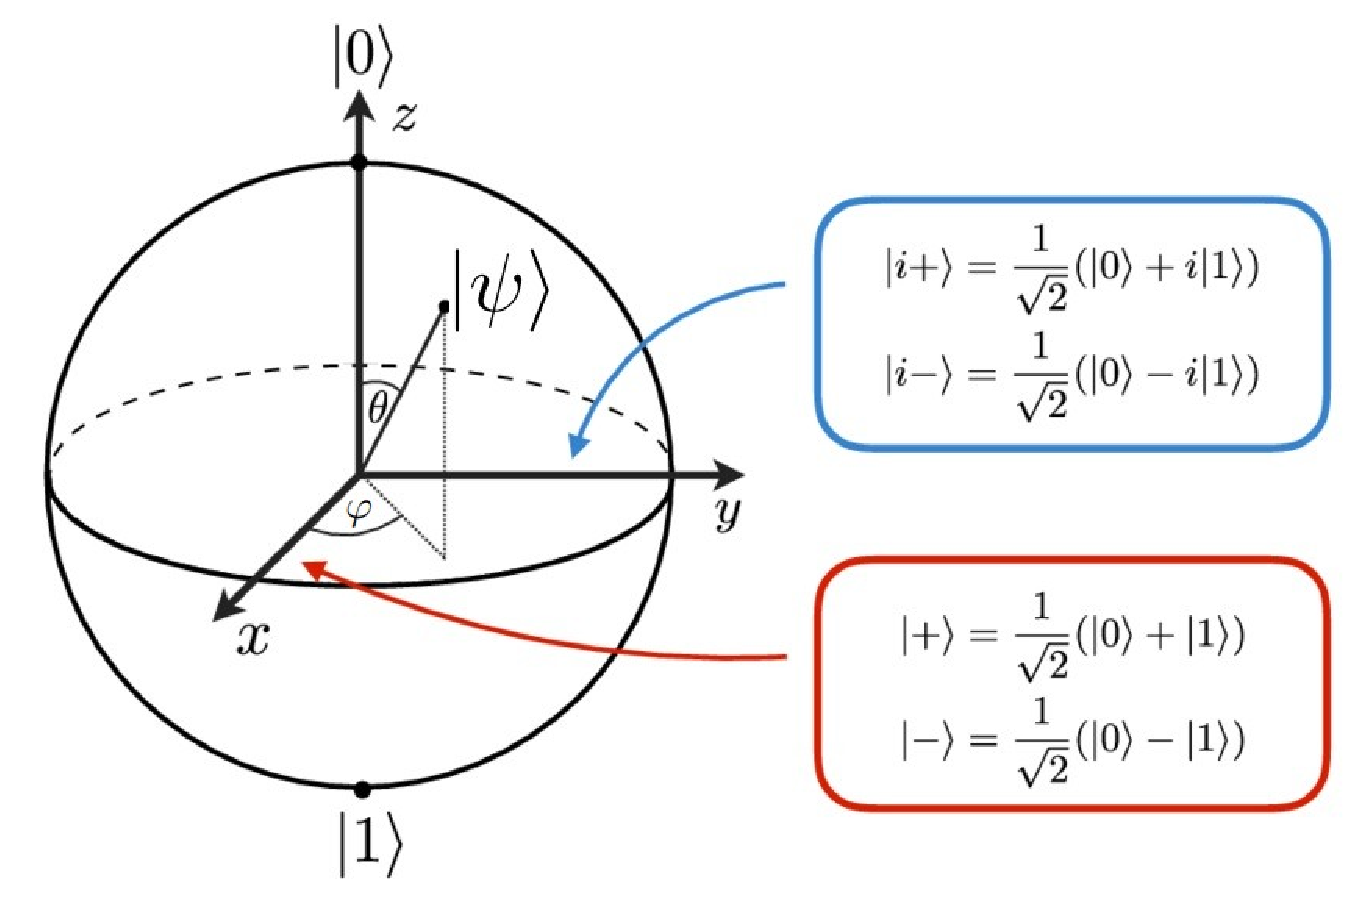
\includegraphics[width=0.5\textwidth]{bloch} \centering \caption{Ilustração da esfera de Bloch \cite{phdthesis}.}
\label{fbloch}
\end{figure}

O estado formado por múltiplos qubits é dado diretamente pelo postulado 4, e as medidas definidas pelo postulado 3 utilizadas na computação quântica são medidas projetivas. Um estado importante de dois qubits é o estado de Bell ou par EPR: 
\begin{equation}
\left|\psi'\right\rangle =\frac{1}{\sqrt{2}}\left(\left|00\right\rangle +\left|11\right\rangle \right).
\end{equation}
Esse estado tem a propriedade de que após a medição do primeiro qubit, que tem probabilidade de $1/2$ para cada resultado, o segundo está definido e será sempre igual ao primeiro resultado. Portanto dizemos que o resultado está correlacionado, e essa correlação é mais forte do que jamais poderia existir entre sistemas clássicos. O estado quântico de um sistema com $n$ qubits é determinado por $2^{n}$ amplitudes. Para $n=500$ há mais amplitudes que átomos no universo, informação que é impossível ser armazenada em um computador clássico. Porém a natureza manipula essa enorme quantidade de dados.

\subsection{Operadores unitários de qubit }

Já discutimos que o conceito fundamental da computação quântica são os vetores de estado chamados qubits e a base no espaço de Hilbert é a base computacional (postulado 1). As medidas realizadas na computação quântica são medidas projetivas (postulado 3) e qubits individuais podem compor um sistema maior de múltiplos qubits (postulado 4), porém nos falta descrever de como o sistema evolui no tempo (postulado 2), e isto é feito com operadores unitários.

Mudanças que ocorrem em um estado quântico genérico podem ser descritas usando a linguagem da computação quântica, que de uma maneira análoga a um computador clássico que é construído por um circuito elétrico, um computador quântico é construído a partir de um circuito quântico contendo operadores quânticos para carregar e manipular a informação quântica.

O operador clássico NOT é definido pela tabela verdade onde $0\rightarrow1$ e $1\rightarrow0$. Podemos construir um análogo quântico, porém sem esquecer que comportamento linear é uma propriedade geral da Mecânica Quântica bem motivada empiricamente, o comportamento não linear poderia levar a aparente paradoxos. Um meio conveniente de representar um operador NOT quântico é na forma matricial: 
\begin{equation}
X\equiv\left[\begin{array}{cc}
0 & 1\\
1 & 0
\end{array}\right].
\end{equation}
E se o estado quântico $\alpha\left|0\right\rangle +\beta\left|1\right\rangle $, que pode ser denotado vetorialmente como $\left[\begin{array}{cc}
\alpha & \beta\end{array}\right]^{T},$ então:

\begin{equation}
X\left[\begin{array}{c}
\alpha\\
\beta
\end{array}\right]=\left[\begin{array}{c}
\beta\\
\alpha
\end{array}\right].
\end{equation}
O que resulta em um comportamento análogo ao NOT clássico, $\alpha\rightarrow\beta$ e $\beta\rightarrow\alpha$. Então a evolução de sistemas quânticos de um único qubit pode ser descrita por operadores unitários ($U^{\dagger}U=I$) que possuem uma descrição matricial por matrizes $2\times2$ . É válido aqui relembrar que qualquer matriz unitária é válida.

Apesar de haver infinitas matrizes $2\times2$, um operador unitário de um qubit arbitrário pode ser decomposto como produto de rotações em diferentes planos e um deslocamento de fase global (uma constante multiplicando como $e^{i\alpha}$). Isso é, uma matriz unitária $2\times2$ arbitrária pode ser decomposta como: 
\begin{equation}
U=e^{i\alpha}\left[\begin{array}{cc}
e^{-i\beta/2} & 0\\
0 & e^{i\beta/2}
\end{array}\right]\left[\begin{array}{cc}
\cos\left(\frac{\gamma}{2}\right) & -\sin\left(\frac{\gamma}{2}\right)\\
\sin\left(\frac{\gamma}{2}\right) & \cos\left(\frac{\gamma}{2}\right)
\end{array}\right]\left[\begin{array}{cc}
e^{-i\delta/2} & 0\\
0 & e^{i\delta/2}
\end{array}\right].
\end{equation}
Onde $\alpha$,$\beta$, $\gamma$ e $\delta$ são valores reais. Essa é uma prescrição exata para qualquer operador unitário de um qubit. Não precisamos ser capazes de trabalharmos com esses operadores para valores arbitrários, podemos construir aproximações arbitrariamente boas para esses operadores usando somente alguns valores especiais fixos. Então uma computação arbitrária de um único qubit pode ser feita com um conjunto finito de operadores, e mais geral ainda, uma computação arbitrária de qualquer número de qubits pode ser gerada com um conjunto finito de operadores que são considerados universais para a computação quântica. Para obter esse conjunto universal, precisamos ver operadores para múltiplos qubits.

\subsection{Operadores de múltiplo qubits}

O protótipo dos operadores lógicos quânticos de múltiplos qubits, é o CNOT (NOT Controlado, que também é chamado de X controlado, ou CX). A ação do operador é descrita a seguir. O operador tem duas entradas, se o qubit de controle é $0$, o qubit alvo permanece inalterado, mas se o qubit de controle é 1, o qubit alvo é invertido, isto é:

\begin{equation}
\begin{split}\left|00\right\rangle \rightarrow\left|00\right\rangle ,\\
\left|01\right\rangle \rightarrow\left|01\right\rangle ,\\
\left|10\right\rangle \rightarrow\left|11\right\rangle ,\\
\left|11\right\rangle \rightarrow\left|10\right\rangle .
\end{split}
\end{equation}
Outra maneira de descrever, é como uma generalização do operador clássico XOR: $\left|A,B\right\rangle \rightarrow\left|A,A\oplus B\right\rangle $, onde $\oplus$ é uma adição de módulo 2. Sua representação matricial é dada por: 
\begin{equation}
U_{CN}=\left[\begin{array}{cccc}
1 & 0 & 0 & 0\\
0 & 1 & 0 & 0\\
0 & 0 & 0 & 1\\
0 & 0 & 1 & 0
\end{array}\right].
\end{equation}
Conforme determinado pelo postulado 2, $U_{CN}$ é um operador unitário. Operadores unitários de qubits e CNOT são os protótipos para todos os outros operadores. Então qualquer operador lógico de múltiplos qubits pode ser construído utilizando CNOT e operadores unitários de 1 qubit. Isso é análogo à universalidade do operador NAND na computação clássica. Porém nem todas operações clássicas possuem análogos quânticos diretos como o NOT. O NAND, por exemplo, é irreversível, ou seja, há uma perda de informação inevitável. Porém operadores quânticos são sempre inversíveis.

A escolha de $\left|0\right\rangle $ e $\left|1\right\rangle $ como base computacional representa somente uma das muitas possíveis escolhas de base de estados para um qubit. Porém a Mecânica Quântica permite maior versatilidade, sendo possível trabalharmos com outras bases.

\subsection{Circuitos quânticos}

Circuitos quânticos são lidos da esquerda para a direita correspondendo a passagem do tempo. Cada linha representa um qubit ao longo do tempo. É convencional assumir que o estado de entrada do circuito consiste de todos qubits em $\left|0\right\rangle $. %Um circuito simples e útil é o responsável por realizar a operação conhecida como swap: trocar o estado entre dois qubits. 

Como sugerido anteriormente, tem algumas características de circuitos clássicos que não estão presentes em circuitos quânticos: Primeiro de tudo, não há loops, circuitos quânticos são acíclicos. Também temos que as linhas não podem ser condensadas (operação conhecida como FANIN em circuitos clássicos). E por fim, também não pode ser feito cópias dos bits (operação conhecida como FANOUT). Antes de avançar, é conveniente introduzirmos uma nova notação: Qubits de controle são identificados como pontos pretos, e medidas são representados por um medidor. Como o nome sugere, essa operação representa uma medição, ou seja, converte o estado $\left|\psi\right\rangle =\alpha\left|0\right\rangle +\beta\left|1\right\rangle $ de um único qubit em um bit probabilístico clássico (que é diferenciado de um qubit por uma linha dupla) onde é $0$ com probabilidade $\left|\alpha\right|^{2}$ e $1$ com probabilidade $\left|\beta\right|^{2}$.

\begin{figure}[ht]
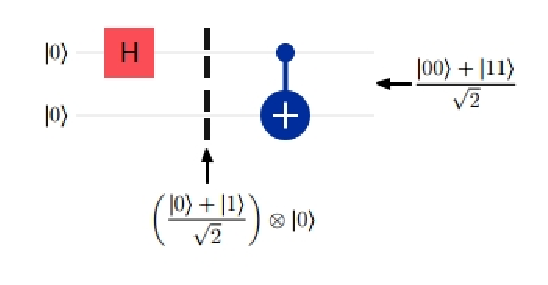
\includegraphics[width=0.5\textwidth]{par_epr} \centering \caption{Circuíto quântico que resulta em um estado Bell.}
\label{bell}
\end{figure}


\subsubsection{Exemplo: Estado de Bell}

Podemos construir um estado de Bell em um sistema com 2 qubits, aplicando um operador Hadamard no primeiro qubit, e então usando este mesmo qubit de controle para um CNOT que tem como alvo o segundo qubit. Sendo o operador de Hadamard responsável por criar sobreposição, ele é definido como 
\begin{equation}
\begin{split}H & \equiv\left[\begin{array}{cc}
1 & 1\\
1 & -1
\end{array}\right]\frac{1}{\sqrt{2}}\end{split}
.
\end{equation}
Para o estado inicial $\left|00\right\rangle $ após aplicarmos o operador Hadamard, o estado do sistema vai para $\left(\left|0\right\rangle +\left|1\right\rangle \right)\left|0\right\rangle /\sqrt{2}$, e então com o CNOT ficamos com $\left(\left|00\right\rangle +\left|11\right\rangle \right)/\sqrt{2}$. Este estado é conhecido como estado de Bell (ou estado EPR, ou ainda par EPR) e está ilustrado na figura \ref{bell}.

\subsubsection{Exemplo: Teleportação quântica}

Teleportação quântica é uma técnica para mover estados quânticos, mesmo sem enviar os qubits diretamente. Muitas ideias da computação quântica são entendidas melhor usando metáforas envolvendo duas partes, popularmente chamadas de Alice e Bob. Então a questão pode ser formulada da seguinte maneira: temos um par de qubits no estado de Bell, Alice e Bob possuem cada um qubit desse par e encontram-se separados. Alice tem a missão de entregar um qubit $\left|\psi\right\rangle =\alpha\left|0\right\rangle +\beta\left|1\right\rangle $ ao Bob, porém ela não conhece o estado do qubit e só pode enviar informação clássica ao Bob.

Isso pode ser feito da maneira descrita a seguir, lembrando que o sistema todo é composto de três qubits, o $\left|\psi\right\rangle $ que Alice deseja enviar para Bob e o par $\left|\beta_{00}\right\rangle $ compartilhado entre ambos. O estado inicial $\left|\psi_{0}\right\rangle $ é então: 
\begin{equation}
\begin{split}\left|\psi_{0}\right\rangle  & =\left|\psi\right\rangle \left|\beta_{00}\right\rangle \\
 & =\left[\alpha\left|0\right\rangle \left(\left|00\right\rangle +\left|11\right\rangle \right)+\beta\left|1\right\rangle \left(\left|00\right\rangle +\left|11\right\rangle \right)\right]\frac{1}{\sqrt{2}}.
\end{split}
\end{equation}
Convenientemente, vamos denotar que os primeiros dois qubits à esquerda pertencem a Alice e o terceiro ao Bob. Então Alice aplica um operador CNOT nos seus dois qubits, usando o qubit que quer enviar como o qubit de controle. Temos assim: 
\begin{equation}
\left|\psi_{1}\right\rangle =\left[\alpha\left|0\right\rangle \left(\left|00\right\rangle +\left|11\right\rangle \right)+\beta\left|1\right\rangle \left(\left|10\right\rangle +\left|01\right\rangle \right)\right]\frac{1}{\sqrt{2}}.
\end{equation}
O próximo passo da Alice é aplicar o operador Hadamard no primeiro qubit: 
\begin{equation}
\begin{split}\left|\psi_{2}\right\rangle  & =\frac{1}{2}\left[\left|00\right\rangle \left(\alpha\left|0\right\rangle +\beta\left|1\right\rangle \right)+\left|01\right\rangle \left(\alpha\left|1\right\rangle +\beta\left|0\right\rangle \right)+\left|10\right\rangle \left(\alpha\left|0\right\rangle -\beta\left|1\right\rangle \right)+\left|11\right\rangle \left(\alpha\left|1\right\rangle -\beta\left|0\right\rangle \right)\right]\end{split}
.\label{psi2A}
\end{equation}
Nota-se que a expressão se divide em 4 termos. No primeiro termo, Alice possui os qubits no estado $\left|00\right\rangle $ e Bob no estado $\alpha\left|0\right\rangle +\beta\left|1\right\rangle $, analisando de maneira similar os outros termos: 
\begin{equation}
\begin{split}\left|00\right\rangle \rightarrow\psi_{3}\equiv\alpha\left|0\right\rangle +\beta\left|1\right\rangle ,\\
\left|01\right\rangle \rightarrow\psi_{3}\equiv\alpha\left|1\right\rangle +\beta\left|0\right\rangle ,\\
\left|10\right\rangle \rightarrow\psi_{3}\equiv\alpha\left|0\right\rangle -\beta\left|1\right\rangle ,\\
\left|11\right\rangle \rightarrow\psi_{3}\equiv\alpha\left|1\right\rangle -\beta\left|0\right\rangle .
\end{split}
\end{equation}
Então uma vez que Bob saiba qual foi a medida da Alice (fato que impede que a informação seja transmitida mais rápido que a luz), ele pode ``corrigir'' seu estado e recuperar $\left|\psi\right\rangle $ aplicando um operador unitário apropriado. Já vimos que para o caso $\left|00\right\rangle $ não é necessário aplicar nenhuma operação (ou aplicar o operador identidade), de maneira análoga para os outros casos: 
\begin{equation}
\begin{split}\left|00\right\rangle  & \rightarrow\mathbb{I},\\
\left|01\right\rangle  & \rightarrow X,\\
\left|10\right\rangle  & \rightarrow Z,\\
\left|11\right\rangle  & \rightarrow ZX.
\end{split}
\end{equation}
Onde o operador $Z$ é definido como: 
\begin{equation}
\begin{split}Z & \equiv\left[\begin{array}{cc}
1 & 0\\
0 & -1
\end{array}\right]\end{split}
.
\end{equation}
Então Bob precisa de maneira genérica aplicar o operador $Z^{M_{1}}X^{M_{2}}$, onde $M_{i}$ indica o bit $i$ na string $\left|bb\right\rangle $ (contando da esquerda para a direita).

\section{Algoritmo quântico}

\subsection{Computação clássica em um computador quântico}

Qualquer circuito clássico pode ser substituído por um circuito equivalente somente com elementos reversíveis, usando um operador conhecido como porta de Toffoli. O operador de Toffoli tem três bits, porém o terceiro bit (bit alvo) é invertido somente se os outros dois bits (bits de controle) são 1, $\left(a,b,c\right)\rightarrow\left(a,b,c\oplus ab\right)$. Operador Toffoli pode ser usado pra simular operadores NAND, FANOUT. Com isso podemos simular qualquer circuito clássico com um circuito reversível equivalente. Se desejamos simular um computador clássico não determinístico, isto é, com a habilidade de gerar bits aleatórios, preparamos um qubit no estado $\left|0\right\rangle $ e usamos um operador de Hadamard, após a medição ser realizada, tem 50/50 de probabilidade de medir $\left|0\right\rangle $ ou $\left|1\right\rangle $.

Porém a habilidade de simular computadores clássicos é apenas uma característica dos computadores quânticos. Funções muito mais poderosas podem ser computadas usando qubits e operadores quânticos, como veremos nas seções a seguir.

% POSSO INSERIR AQUI O PROBLEMA DA LINEARIDDE ?

\subsection{Paralelismo quântico}

De forma simplificada, o paralelismo quântico permite que computadores quânticos avaliem a função $f\left(x\right)$ para diferentes valores de $x$ simultaneamente. Isto é, supondo uma função com o domínio e imagem de um bit ( $f\left(x\right):\left\{ 0,1\right\} \rightarrow\left\{ 0,1\right\} $), uma maneira conveniente de computar essa função é considerar um computador quântico de dois qubits que inicia no estado $\left|x,y\right\rangle $ e com uma sequência de operadores então termina no estado $\left|x,y\oplus f\left(x\right)\right\rangle $.

Vamos chamar o operador responsável pela transformação $\left|x,y\right\rangle \rightarrow\left|x,y\oplus f\left(x\right)\right\rangle $, de $U_{f}$, e o primeiro registo de dado, e o segundo de alvo. Se $y=0$, então o estado final é simplesmente $\left|x,f\left(x\right)\right\rangle $. Considerando então um sistema onde foi aplicado o operador de Hadamard no primeiro qubit, o estado é então $\frac{1}{\sqrt{2}}\left(\left|0,0\right\rangle +\left|1,0\right\rangle \right)$, e após aplicar o operador $U_{f}$ temos: 
\begin{equation}
\frac{1}{\sqrt{2}}\left(\left|0,f\left(0\right)\right\rangle +\left|1,f\left(1\right)\right\rangle \right).
\end{equation}
Os diferentes termos contém informações de $f\left(0\right)$ e $f\left(1\right)$. Dessa forma é como se tivéssemos avaliados $f\left(x\right)$ simultaneamente para ambos os valores de $x$. Esse processo pode ser generalizado para funções de quantidades arbitrárias de bits, usando uma operação geral chamada de transformada de Hadamard (ou Walsh-Hadamard). Esta transformada não é nada além de $n$ operadores Hadamard atuando paralelamente em $n$ qubits ($H^{\otimes n}$).

Então, o paralelismo quântico de uma função de $n$ bits de entrada e um bit de saída, pode ser feito da seguinte maneira: 
\begin{enumerate}
\item Preparamos o estado de $n+1$ qubits: $\left|0\right\rangle ^{\otimes n}\left|0\right\rangle $ ; 
\item Aplicamos o Hadamard paralelo aos $n$ qubits: $\frac{1}{\sqrt{2^{n}}}\sum_{x}\left|x\right\rangle \left|0\right\rangle $; 
\item Implementamos $U_{f}$ :$\frac{1}{\sqrt{2^{n}}}\sum_{x}\left|x\right\rangle \left|f\left(x\right)\right\rangle $. 
\end{enumerate}
Porém a medição nos retorna apenas um dos resultados de $f\left(x\right)$, para um único valor de $x$. Dessa maneira a computação quântica requer mais do que apenas paralelismo quântico, precisamos extrair informação de mais do que um valor de $f\left(x\right)$. Vvamos ver dois exemplos de como isso pode ser feito.

\subsection{Algoritmo de Deutsch}

A versão que vamos abordar é uma versão simplificada e melhorada da versão original \cite{nielsen2000quantum}. Como feito anteriormente, primeiro usamos o operador de Hadamard para preparar o primeiro qubit ($x$) em um estado de superposição: $\left(\left|0\right\rangle +\left|1\right\rangle \right)\frac{1}{\sqrt{2}}$, mas agora preparamos o segundo qubit ($y$) também em uma superposição: $\left(\left|0\right\rangle -\left|1\right\rangle \right)/\frac{1}{\sqrt{2}}$ , o que pode ser feito aplicando o Hadamard em um estado $\left|1\right\rangle $. Então considerando o seguinte estado inicial: 
\begin{equation}
\left|\psi_{0}\right\rangle =\left(\left|0\right\rangle \right)\otimes\left(\left|1\right\rangle \right).\label{anterior0}
\end{equation}
Temos, depois de aplicar o operador Hadamard em ambos os qubits: 
\begin{equation}
\begin{split}\left|\psi_{1}\right\rangle  & =\left[\frac{\left(\left|0\right\rangle +\left|1\right\rangle \right)}{\sqrt{2}}\right]\otimes\left[\frac{\left(\left|0\right\rangle -\left|1\right\rangle \right)}{\sqrt{2}}\right]\\
 & =\sum_{x\in\left\{ 0,1\right\} ^{1}}\left[\frac{\left|x\right\rangle }{\sqrt{2}}\left(\frac{\left|0\right\rangle -\left|1\right\rangle }{\sqrt{2}}\right)\right].
\end{split}
\label{anterior}
\end{equation}
Aplicando o operador responsável pela transformação $\left|x,y\right\rangle \rightarrow\left|x,y\oplus f\left(x\right)\right\rangle $ obtemos: 
\begin{equation}
\begin{split}\left|\psi_{2}\right\rangle  & =\left[\left|0\right\rangle \left(\left|0\oplus f\left(0\right)\right\rangle -\left|1\oplus f\left(0\right)\right\rangle \right)+\left|1\right\rangle \left(\left|0\oplus f\left(1\right)\right\rangle -\left|1\oplus f\left(1\right)\right\rangle \right)\right]\frac{1}{2}\\
 & =\left[\left|0\right\rangle \left(\left|f\left(0\right)\right\rangle -\left|1\oplus f\left(0\right)\right\rangle \right)+\left|1\right\rangle \left(\left|f\left(1\right)\right\rangle -\left|1\oplus f\left(1\right)\right\rangle \right)\right].\frac{1}{2}
\end{split}
\end{equation}
Agora precisamos analisar as diferentes combinações possíveis de valores para $f\left(0\right)$ e $f\left(1\right)$. Começando com o caso em que $f\left(0\right)=f\left(1\right)$: 
\begin{equation}
\left|\psi_{2}\right\rangle =\left\{ \begin{array}{cc}
\left[+\left|0\right\rangle \left(\left|0\right\rangle -\left|1\right\rangle \right)+\left|1\right\rangle \left(\left|0\right\rangle -\left|1\right\rangle \right)\right]\frac{1}{2}, & f\left(0\right)=0\\
\left[-\left|0\right\rangle \left(\left|0\right\rangle -\left|1\right\rangle \right)-\left|1\right\rangle \left(\left|0\right\rangle -\left|1\right\rangle \right)\right]\frac{1}{2}, & f\left(0\right)=1
\end{array}\right..
\end{equation}
O segundo conjunto de situações é quando $f\left(0\right)\neq f\left(1\right)$: 
\begin{equation}
\left|\psi_{2}\right\rangle =\left\{ \begin{array}{cc}
\left[+\left|0\right\rangle \left(\left|0\right\rangle -\left|1\right\rangle \right)-\left|1\right\rangle \left(\left|0\right\rangle -\left|1\right\rangle \right)\right]\frac{1}{2}, & f\left(0\right)=0\\
\left[-\left|0\right\rangle \left(\left|1\right\rangle -\left|0\right\rangle \right)+\left|1\right\rangle \left(\left|0\right\rangle -\left|1\right\rangle \right)\right]\frac{1}{2}, & f\left(0\right)=1
\end{array}\right..
\end{equation}
Podemos generalizar então: 
\begin{equation}
\begin{split}\left|\psi_{2}\right\rangle  & =\left[\left(-1\right)^{f\left(0\right)}\left|0\right\rangle \left(\left|0\right\rangle -\left|1\right\rangle \right)+\left(-1\right)^{f\left(1\right)}\left|1\right\rangle \left(\left|0\right\rangle -\left|1\right\rangle \right)\right]\frac{1}{2}\\
 & =\sum_{x\in\left\{ 0,1\right\} ^{1}}\left[\frac{\left(-1\right)^{f\left(x\right)}\left|x\right\rangle }{\sqrt{2}}\left(\frac{\left|0\right\rangle -\left|1\right\rangle }{\sqrt{2}}\right)\right]
\end{split}
.\label{anterior1}
\end{equation}
Estado que tem a seguinte representação vetorial: 
\begin{equation}
\left|\psi_{2}\right\rangle =\left[\begin{array}{cccc}
\left(-1\right)^{f\left(0\right)} & -\left(-1\right)^{f\left(0\right)} & \left(-1\right)^{f\left(1\right)} & -\left(-1\right)^{f\left(1\right)}\end{array}\right]^{T}\frac{1}{2}.
\end{equation}
Agora vamos aplicar o Hadamard no primeiro qubit. Lembrando que para um espaço de $2$ qubits precisamos então fazer um produto tensorial com uma matriz identidade: 
\begin{equation}
H\left(0\right)=\frac{1}{\sqrt{2}}\left[\begin{array}{cc}
1 & 1\\
1 & -1
\end{array}\right]\otimes\left[\begin{array}{cc}
1 & 0\\
0 & 1
\end{array}\right]=\left[\begin{array}{cccc}
1 & 0 & 1 & 0\\
0 & 1 & 0 & 1\\
1 & 0 & -1 & 0\\
0 & 1 & 0 & -1
\end{array}\right]\frac{1}{\sqrt{2}}.
\end{equation}
Então aplicando: 
\begin{equation}
\left|\psi_{3}\right\rangle =\frac{1}{\sqrt{2}}\left[\begin{array}{cccc}
1 & 0 & 1 & 0\\
0 & 1 & 0 & 1\\
1 & 0 & -1 & 0\\
0 & 1 & 0 & -1
\end{array}\right]\left[\begin{array}{c}
\left(-1\right)^{f\left(0\right)}\\
-\left(-1\right)^{f\left(0\right)}\\
\left(-1\right)^{f\left(1\right)}\\
-\left(-1\right)^{f\left(1\right)}
\end{array}\right]\frac{1}{2}=\left[\begin{array}{c}
\left(-1\right)^{f\left(0\right)}+\left(-1\right)^{f\left(1\right)}\\
-\left(-1\right)^{f\left(0\right)}-\left(-1\right)^{f\left(1\right)}\\
\left(-1\right)^{f\left(0\right)}-\left(-1\right)^{f\left(1\right)}\\
-\left(-1\right)^{f\left(0\right)}+\left(-1\right)^{f\left(1\right)}
\end{array}\right]\frac{1}{2\sqrt{2}}.
\end{equation}
Temos novamente os 4 casos de valores de $f\left(0\right)$ e $f\left(1\right)$, para analisar. Começando com $f\left(0\right)=f\left(1\right)$: 
\begin{equation}
\begin{split}\left|\psi_{3}\right\rangle  & =\left\{ \begin{array}{cc}
\left[\begin{array}{cccc}
1 & -1 & 0 & 0\end{array}\right]^{T}\frac{1}{\sqrt{2}} & ,f\left(0\right)=0\\
\left[\begin{array}{cccc}
-1 & 1 & 0 & 0\end{array}\right]^{T}\frac{1}{\sqrt{2}} & ,f\left(0\right)=1
\end{array}\right.\\
 & =\left\{ \begin{array}{cc}
+\left(\left|00\right\rangle -\left|01\right\rangle \right)\frac{1}{\sqrt{2}} & ,f\left(0\right)=0\\
-\left(\left|00\right\rangle -\left|01\right\rangle \right)\frac{1}{\sqrt{2}} & ,f\left(0\right)=1
\end{array}\right.\\
 & =\pm\left(\left|00\right\rangle -\left|01\right\rangle \right)\frac{1}{\sqrt{2}}\\
 & =\pm\left|0\right\rangle \left(\left|0\right\rangle -\left|1\right\rangle \right)\frac{1}{\sqrt{2}}.
\end{split}
\end{equation}
E se $f\left(0\right)\neq f\left(1\right)$: 
\begin{equation}
\begin{split}\left|\psi_{3}\right\rangle  & =\left\{ \begin{array}{cc}
\left[\begin{array}{cccc}
0 & 0 & 1 & -1\end{array}\right]^{T}\frac{1}{\sqrt{2}} & ,f\left(0\right)=0\\
\left[\begin{array}{cccc}
0 & 0 & -1 & 1\end{array}\right]^{T}\frac{1}{\sqrt{2}} & ,f\left(0\right)=1
\end{array}\right.\\
 & =\left\{ \begin{array}{cc}
+\left(\left|10\right\rangle -\left|11\right\rangle \right)\frac{1}{\sqrt{2}} & ,f\left(0\right)=0\\
-\left(\left|10\right\rangle -\left|11\right\rangle \right)\frac{1}{\sqrt{2}} & ,f\left(0\right)=1
\end{array}\right.\\
 & =\pm\left(\left|10\right\rangle -\left|11\right\rangle \right)\frac{1}{\sqrt{2}}\\
 & =\pm\left|1\right\rangle \left(\left|0\right\rangle -\left|1\right\rangle \right)\frac{1}{\sqrt{2}}.
\end{split}
\end{equation}
Podemos simplificar o resultado lembrando que: 
\begin{equation}
f\left(0\right)\oplus f\left(1\right)=\left\{ \begin{array}{cc}
0, & f\left(0\right)=f\left(1\right)\\
1, & f\left(0\right)\neq f\left(1\right)
\end{array}\right..
\end{equation}
Então: 
\begin{equation}
\left|\psi_{3}\right\rangle =\pm\left|f\left(0\right)\oplus f\left(1\right)\right\rangle \left(\left|0\right\rangle -\left|1\right\rangle \right)\frac{1}{\sqrt{2}}.
\end{equation}
O sinal $\pm$ é irrelevante, pois a medida será do quadrado dos coeficientes. Dessa maneira podemos determinar a propriedade global $f\left(0\right)\oplus f\left(1\right)$ com apenas uma medida de $f\left(x\right)$, enquanto caso tivéssemos um aparato clássico precisaríamos ao menos de 2 medições. A essência do desenvolvimento de muitos algoritmos quânticos é realizar uma escolha inteligente da função e da transformação final que permita uma determinação eficiente da informação global útil sobre a função, informação essa que não poderia ser obtida rapidamente em um computador clássico.

\subsection{O algoritmo de Deutsch-Jozsa}

O algoritmo de Deutsch é um caso simples de um caso mais geral, que vamos chamar de algoritmo de Deutsch-Jozsa. A aplicação é conhecida como problema de Deustch e pode ser descrito como um jogo:

Os dois protagonistas são Alice em Amsterdam e Bob em Boston, a Alice seleciona um número $x$ entre $0$ e $2^{n}-1$ e envia uma carta para o Bob. Então Bob calcula alguma função $f\left(x\right)$ e responde Alice com o resultado $0$ ou $1$. Porém Bob prometeu usar uma função que é um dos dois tipos: ou $f\left(x\right)$ é constante para todos valores de $x$ ou $f\left(x\right)$ é perfeitamente balanceado, isto é, 0 para exatamente metade dos casos possíveis e 1 para a outra metade. O objetivo da Alice é determinar com certeza se Bob escolheu uma função constante ou balanceada.

No caso clássico, Alice pode enviar ao Bob apenas um valor de $x$ por carta. No pior cenário será necessário ao menos $\frac{2^{n}}{2}+1$ requisições ao Bob, uma vez que pode receber $\frac{2^{n}}{2}$ respostas com o valor $0$ antes de receber uma com o valor $1$ (ou vice-versa). Em cada carta, Alice envia $n$ bits de informação. Mas se podem trocar qubits e Bob usa uma transformação unitária $U_{f}$ para calcular $f\left(x\right)$, Alice pode alcançar seu objetivo com apenas uma correspondência usando o algoritmo que iremos discutir na sequência.

Semelhante ao algoritmo de Deutsch, Alice deve ter $n$ qubits para armazenar $x$ (registradores de dados) e um único qubit no qual o Bob vai guardar a resposta (registrador alvo). Alice vai preparar os qubits em um estado de superposição, então Bob deve avaliar $f\left(x\right)$ usando paralelismo quântico, deixar o resultado no qubit de resposta e devolver a Alice, após isto, Alice então interfere nos estados de superposição usando a transformada de Hadamard nos registradores de dados e termina realizando uma medição adequada para determinar se $f$ é constante ou balanceado.

De forma análoga ao caso anterior, equação (\ref{anterior0}), começamos com o estado inicial: 
\begin{equation}
\left|\psi_{0}\right\rangle =\left|0\right\rangle ^{\otimes n}\left|1\right\rangle .
\end{equation}
Então após aplicarmos os operadores de Hadamard, análogo também à equação (\ref{anterior}): 
\begin{equation}
\left|\psi_{1}\right\rangle =\sum_{x\in\left\{ 0,1\right\} ^{n}}\frac{\left|x\right\rangle }{\sqrt{2^{n}}}\left[\frac{\left|0\right\rangle -\left|1\right\rangle }{\sqrt{2}}\right].
\end{equation}
E como demonstramos anteriormente, na equação (\ref{anterior1}), após aplicarmos o operador $U_{f}$, o estado resultante pode ser generalizado como: 
\begin{equation}
\left|\psi_{2}\right\rangle =\sum_{x\in\left\{ 0,1\right\} ^{n}}\frac{\left(-1\right)^{f\left(x\right)}\left|x\right\rangle }{\sqrt{2^{n}}}\left[\frac{\left|0\right\rangle -\left|1\right\rangle }{\sqrt{2}}\right].
\end{equation}
Nesse momento Alice tem um conjunto de qubits em que o resultado da avaliação da função do Bob está armazenado na amplitude do estado do qubit em superposição. Agora Alice pode usar a interferência nos termos em superposição, usando a transformação de Hadamard nos registradores dados. Antes de calcularmos a aplicação da transformada de Hadamard nos registradores de dados, primeiro vamos calcular a transformada em um único estado $\left|x\right\rangle $. Considerando apenas um qubit: 
\begin{equation}
\begin{split}H\left|0\right\rangle  & =\frac{1}{\sqrt{2}}\left(\left|0\right\rangle +\left|1\right\rangle \right)=\sum_{z\in\left\{ 0,1\right\} ^{1}}\frac{\left|z\right\rangle }{\sqrt{2}},\\
H\left|1\right\rangle  & =\frac{1}{\sqrt{2}}\left(\left|0\right\rangle -\left|1\right\rangle \right)=\sum_{z\in\left\{ 0,1\right\} ^{1}}\left(-1\right)^{z}\frac{\left|z\right\rangle }{\sqrt{2}}.
\end{split}
\end{equation}
Então podemos generalizar para um qubit: 
\begin{equation}
H\left|x\right\rangle =\sum_{z\in\left\{ 0,1\right\} ^{1}}\left(-1\right)^{x\cdot z}\frac{\left|z\right\rangle }{\sqrt{2}}.
\end{equation}
Para 2 qubits, a transformada de Hadamard é dada por: 
\begin{equation}
H^{\otimes2}=\frac{1}{\sqrt{2}}\left[\begin{array}{cc}
1 & 1\\
1 & -1
\end{array}\right]\otimes\left[\begin{array}{cc}
1 & 1\\
1 & -1
\end{array}\right]\frac{1}{\sqrt{2}}=\left[\begin{array}{cccc}
1 & 1 & 1 & 1\\
1 & -1 & 1 & -1\\
1 & 1 & -1 & -1\\
1 & -1 & -1 & 1
\end{array}\right].
\end{equation}
E então: 
\begin{equation}
\begin{split}H^{\otimes2}\left|00\right\rangle  & =\frac{1}{2}\left(\left|00\right\rangle +\left|01\right\rangle +\left|10\right\rangle +\left|11\right\rangle \right)=\sum_{z_{0},z_{1}\in\left\{ 0,1\right\} ^{1}}\frac{\left|z_{0},z_{1}\right\rangle }{{2}},\\
H^{\otimes2}\left|01\right\rangle  & =\frac{1}{2}\left(\left|00\right\rangle -\left|01\right\rangle +\left|10\right\rangle -\left|11\right\rangle \right)=\sum_{z_{0},z_{1}\in\left\{ 0,1\right\} ^{1}}\frac{\left(-1\right)^{z_{1}}\left|z_{0},z_{1}\right\rangle }{2},\\
H^{\otimes2}\left|10\right\rangle  & =\frac{1}{2}\left(\left|00\right\rangle +\left|01\right\rangle -\left|10\right\rangle -\left|11\right\rangle \right)=\sum_{z_{0},z_{1}\in\left\{ 0,1\right\} ^{1}}\frac{\left(-1\right)^{z_{0}}\left|z_{0},z_{1}\right\rangle }{2},\\
H^{\otimes2}\left|11\right\rangle  & =\frac{1}{2}\left(\left|00\right\rangle -\left|01\right\rangle -\left|10\right\rangle +\left|11\right\rangle \right)=\sum_{z_{0},z_{1}\in\left\{ 0,1\right\} ^{1}}\frac{\left(-1\right)^{z_{0}+z_{1}}\left|z_{0},z_{1}\right\rangle }{2}.
\end{split}
\end{equation}
Por sua vez, pode ser generalizado como: 
\begin{equation}
\begin{split}H^{\otimes2}\left|x_{0},x_{1}\right\rangle  & =\sum_{z_{0},z_{1}\in\left\{ 0,1\right\} ^{1}}\frac{\left(-1\right)^{x_{0}\cdot z_{0}+x_{1}\cdot z_{1}}\left|z_{0},z_{1}\right\rangle }{2},\\
H^{\otimes2}\left|x\right\rangle  & =\sum_{z\in\left\{ 0,1\right\} ^{2}}\frac{\left(-1\right)^{x\cdot z}\left|z\right\rangle }{2}.
\end{split}
\end{equation}
Onde $x\cdot z$ é o produto interno bit a bit de $x$ e $z$ com a operação de adição de módulo 2 ($\oplus$). Finalmente, isto pode ser generalizado para $n$ qubits como: 
\begin{equation}
H^{\otimes n}\left|x\right\rangle =\sum_{z\in\left\{ 0,1\right\} ^{n}}\frac{\left(-1\right)^{x\cdot z}\left|z\right\rangle }{\sqrt{2^{n}}}.
\end{equation}
Então: 
\begin{equation}
\begin{split}\left|\psi_{3}\right\rangle  & =H^{\otimes n}\left|\psi_{2}\right\rangle \\
 & =\sum_{x,z\in\left\{ 0,1\right\} ^{n}}\frac{\left(-1\right)^{x\cdot z+f\left(x\right)}\left|z\right\rangle }{2^{n}}\left[\frac{\left|0\right\rangle -\left|1\right\rangle }{\sqrt{2}}\right]
\end{split}
.
\end{equation}
A amplitude para o estado $\left|0\right\rangle ^{\otimes n}$ dos qubits do registrador de dados ( $z=0\dots0$) é $\alpha_{0}=\sum_{x\in\left\{ 0,1\right\} ^{n}}\frac{\left(-1\right)^{f\left(x\right)}}{2^{n}}$. Agora vamos analisar os dois casos, quando $f\left(x\right)$ é constante e quando é perfeitamente equilibrada. Se $f\left(x\right)$ é constante constante, nesse caso, para qualquer $x$ que tenha sido requisitado , $f\left(x\right)=c,$ e como temos $2^{n}$ termos: 
\begin{equation}
\alpha_{0}=\sum_{x\in\left\{ 0,1\right\} ^{n}}\frac{\left(-1\right)^{0}}{2^{n}}=1\quad\text{ou}\quad\alpha_{0}=\sum_{x\in\left\{ 0,1\right\} ^{n}}\frac{\left(-1\right)^{1}}{2^{n}}=-1.
\end{equation}
Independente do sinal, como o tamanho do vetor deve ser unitário, então todas as outras amplitudes devem ser necessariamente $0$. Agora se $f\left(x\right)$ é perfeitamente balanceado, metade dos termos do somatório vai ser $+1$ e metade $-1$, então como resultado final temos $\alpha_{0}=0$. Dessa forma, a medida vai levar a algum outro resultado com ao menos um bit diferente de $0$ nos registradores de dados. Podemos concluir então que se o estado medido por Alice for $\left|0\right\rangle ^{\otimes n}$, a função é constante, se não, é balanceada.

Dessa forma mostra-se que o computador quântico pode resolver o problema de Deutsch apenas com uma avaliação da função $f$, comparado a $\frac{2^{n}}{2}+1$ avaliações clássicas necessárias. Porém há alguns problemas, dentre eles podemos citar que não há aplicação conhecida do problema e se a Alice pudesse usar um computador probabilístico, ela resolveria o problema muito rapidamente com uma boa probabilidade.

Porém, antes de concluirmos a discussão sobre algoritmos quânticos, precisamos lembrar da presença de ruídos em dispositivos reais, isto é, uma perturbação no valor medido quando em comparação com o valor esperado em uma situação ideal . Isto decorre do fato de que quando não lidamos com sistemas ideais, as observações sofrem interferência, pois o mundo real não é um sistema perfeitamente fechado. Desta maneira, sistemas reais sofrem interações indesejadas com o mundo exterior \cite{nielsen2000quantum}.

\bibliographystyle{plain}
\bibliography{referencias}

\end{document}
